\chapter{从局域守恒到爱因斯坦场方程}

爱因斯坦场方程简单到可以写在一行里，但展开成分量却出了名地令人不快。一个度规有许多克里斯托费尔符号；克里斯托费尔符号包含度规的导数；而曲率张量既包含克里斯托费尔符号的导数，也包含它们的乘积。甚至在尝试求解任何东西之前，计算就可能占满好几页。对于某个特定的度规，符号计算软件往往是管理这种记账工作的明智方式。

原理比计算要干净得多。因此，我们不会一开始就逐个分量地攻击这些方程。我们要问的是，引力需要什么样的方程。论证从牛顿理论出发，经过局域守恒，最后发现曲率张量的唯一一种组合，它能够一致地等于能量与动量的流和密度。整章中我们使用\(c=1\)。

\section{牛顿式的双向通道}

引力有两条互补的指令。引力场告诉物质如何运动，而物质告诉引力场应该是什么。这条双向通道在牛顿力学中已经可见。

设\(\phi(\mathbf{x},t)\)为牛顿引力势。一个质量为\(m\)的检验物体感受到力
\begin{equation}
 \mathbf{F}=-m\nabla\phi.
\end{equation}
把它与\(\mathbf{F}=m\mathbf{a}\)结合，检验质量被消去：
\begin{equation}
 \mathbf{a}=-\nabla\phi.
\end{equation}
这是这条通道的第一个方向。一旦场已知，它就告诉每一个自由落体如何加速，与该物体的质量无关。

相反的方向是泊松方程，
\begin{equation}
 \nabla^2\phi=4\pi G\rho,
 \qquad
 \nabla^2=
 \frac{\partial^2}{\partial x^2}
 +\frac{\partial^2}{\partial y^2}
 +\frac{\partial^2}{\partial z^2},
 \label{eq:poisson}
\end{equation}
其中\(\rho(\mathbf{x},t)\)是单位体积的质量。因子\(4\pi\)本可以并入\(G\)的定义中，但它只会在别处重新出现。方程~\eqref{eq:poisson}说明，物质的分布是势的源。

对于一个总质量为\(M\)的球对称物体，外部解为
\begin{equation}
 \phi(r)=-\frac{GM}{r}.
 \label{eq:newton-potential}
\end{equation}
密度可以集中在中心附近，可以均匀分布，也可以向表面平滑地逐渐减小。球对称性和总质量就是外部解所记得的全部内容。在物质外部，\(\nabla^2\phi=0\)；对\(1/r\)求导便给出平方反比力。如果我们只关心外部，我们可以把源缩小为一个点，并在除该点以外的各处使用同一表达式。

\begin{classroomqa}
\audiencequestion{球体内部的密度必须为常数，然后在其边界处不连续地跳到零吗？}
\lecturerresponse{不。对于这个论证，它必须是球对称的，但它不必是常数，也不必跳跃。它可以平滑地减小到零。这些内部细节都不会改变外部势，外部势只依赖于总质量。
\lecturetimestamp{00:09:13--00:09:37}}
\end{classroomqa}

这种场表述看起来比遥远质量之间的直接力更局域，但牛顿引力仍然包含瞬时超距作用。移动源，牛顿势就立刻在各处改变。广义相对论必须既替换这种瞬时响应，也替换力定律。

\section{一个弱场线索，还不是方程}

第一条指令的相对论版本已经知道：一旦给定时空度规，自由落体粒子就沿时空测地线运动。我们现在需要泊松方程的相对论替代品，即物质决定度规的那条指令。

施瓦西几何提供了一个线索。它的时间-时间分量为
\begin{equation}
 g_{00}=1-\frac{2GM}{r}.
\end{equation}
利用方程~\eqref{eq:newton-potential}，这变为
\begin{equation}
 g_{00}=1+2\phi.
\end{equation}
因此，
\begin{equation}
 \nabla^2g_{00}=2\nabla^2\phi=8\pi G\rho.
 \label{eq:weak-mnemonic}
\end{equation}

方程~\eqref{eq:weak-mnemonic}必须打折扣地看待。它是一个助记式，不是爱因斯坦方程。它使用度规的一个特殊分量和一个非相对论源。尽管如此，它展示了我们正在寻找的那种质地：一边是物质密度，另一边是几何的二阶导数。它是从泊松方程通向协变场方程的粗略桥梁。

右边现在需要更仔细地考察。在相对论单位中质量就是能量，所以\(\rho\)首先应被理解为能量密度。但能量密度并不是一个完整的相对论对象。为了看清伴随它的是什么，我们从一个更简单的守恒量开始。

\section{电荷密度、电流与局域守恒}

设\(Q\)为电荷，并设\(\sigma\)表示电荷密度：
\begin{equation}
 \sigma=\lim_{\Delta V\to0}\frac{\Delta Q}{\Delta V}.
\end{equation}
密度问的是在某一瞬间有多少电荷占据一个小空间体积。电流问的是另一个问题。在空间中放置一个无穷小的有向窗口，数一数每单位面积每单位时间有多少电荷穿过它。三种可能的方向给出空间电流分量\(J^i\)。

量纲比较很有启发性。电荷密度是电荷除以三个空间长度。电流是电荷除以两个空间长度和一个时间间隔。当\(c=1\)时，时间和长度具有相同的单位，因此密度和电流具有匹配的量纲。它们作为四维矢量组合在一起：
\begin{equation}
 J^\mu=(J^0,J^1,J^2,J^3),
 \qquad J^0=\sigma.
\end{equation}

电荷守恒不仅仅是说宇宙中的总电荷保持不变。它是局域的。电荷不可能从教室里消失并瞬间在比邻星重新出现。如果它离开一个区域，就必须穿过该区域的边界。对于一个小盒子，内部电荷的减少等于通过其壁面向外的通量。高斯定理给出
\begin{equation}
 \dot{\sigma}+\nabla\cdot\mathbf{J}=0,
\end{equation}
或者，使用求和约定，
\begin{equation}
 \partial_\mu J^\mu=0.
 \label{eq:charge-continuity}
\end{equation}
在弯曲坐标中，相应的张量方程用协变导数写出：
\begin{equation}
 D_\mu J^\mu=0.
\end{equation}
协变导数的目的不是装饰。它使这一陈述在任何坐标系中都有意义。

\section{为什么能量和动量需要两个指标}

电荷本身是不变量。相对运动的观察者对于电子的电荷意见一致，尽管他们对于电荷密度或电流意见不一致。运动的观察者看到洛伦兹收缩的体积，并且可能在另一个观察者看到静止电荷的地方看到电荷风。因此，尽管总电荷不变，密度和电流在参考系改变下会混合。

能量和动量更为复杂。甚至它们的总量也依赖于参考系。一个观察者可能看到一个静止的粒子，只携带其静止能量而没有空间动量。另一个从旁边走过的观察者则同时看到动能和动量。这四个量构成动量四维矢量
\begin{equation}
 P^\nu=(P^0,P^1,P^2,P^3),
 \qquad P^0=E.
\end{equation}
每个分量\(P^\nu\)都是局域守恒的。因此每个分量都既有密度又有流动。一个指标标识守恒量；第二个指标标识密度或流动方向。

从能量开始。它的密度是\(T^{00}\)。能量也可以穿过一个窗口，因此\(T^{0i}\)是能量在\(x^i\)方向上的流动。现在取动量的\(i\)分量。它的密度是\(T^{i0}\)，它在\(x^j\)方向上的流动是\(T^{ij}\)。在这一约定下：
\begin{itemize}
 \item \(T^{00}\)是能量密度；
 \item \(T^{0i}\)是沿\(i\)方向的能量通量；
 \item \(T^{i0}\)是动量\(i\)分量的密度；
 \item \(T^{ij}\)是\(i\)动量通过垂直于\(j\)的表面的通量。
\end{itemize}
空间块\(T^{ij}\)稍后将被认作应力：其对角元包括压强，而非对角元描述剪切。

\begin{classroomqa}
\audiencequestion{当\(T^{m0}(x)\)被称为动量\(m\)分量的密度时，\(x\)本身是否意味着位置的\(m\)分量？}
\lecturerresponse{不。自变量\(x\)表示密度被求值处的时空位置；它代表所有坐标。指标\(m\)标记正在计数的动量分量。
\lecturetimestamp{00:41:07--00:41:27}}
\end{classroomqa}

对于每个固定的\(\nu\)，局域守恒给出一个连续性方程：
\begin{equation}
 D_\mu T^{\nu\mu}=0.
 \label{eq:stress-continuity}
\end{equation}
\(\nu\)的四个值给出一个能量方程和三个动量方程。密度和流动共同构成能量-动量张量。

\begin{figure}[htbp]
\centering
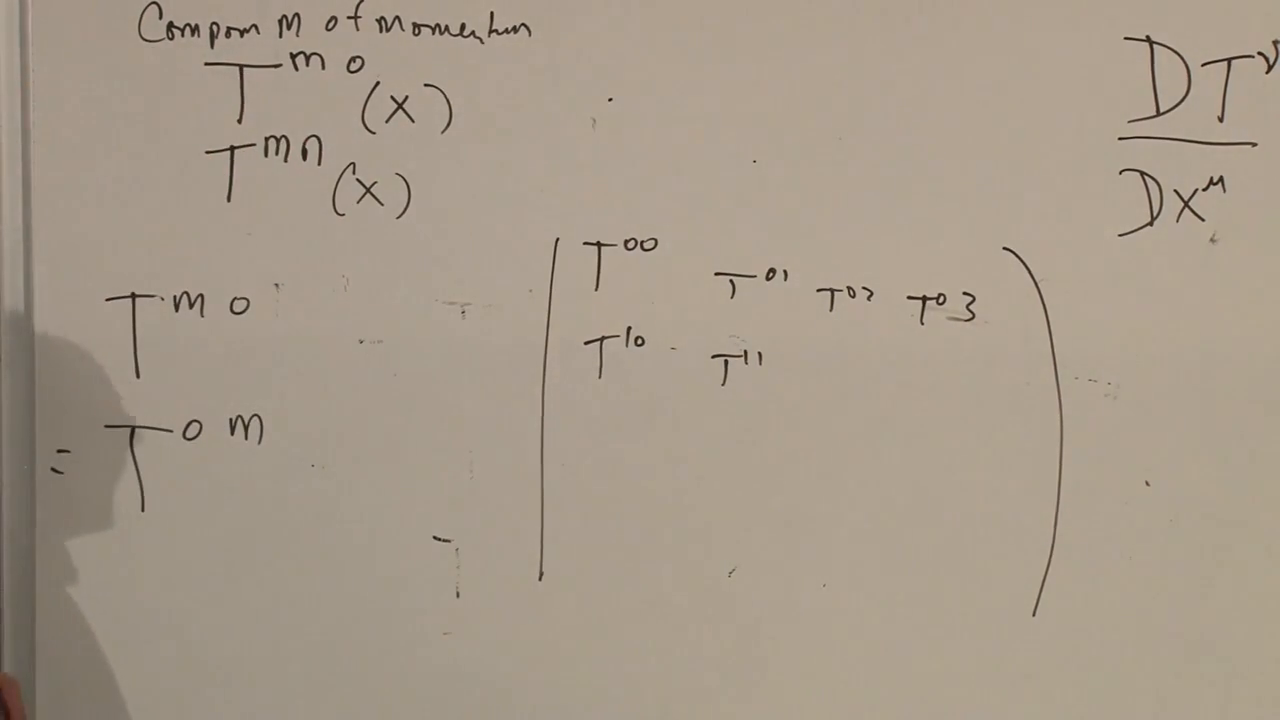
\includegraphics[width=0.84\textwidth]{lecture_09_figure_02.png}
\caption{黑板上正在形成的能量-动量阵列。第一个指标选择能量或某个动量分量；第二个指标选择密度或流动。}
\lectureframe{00:44:30}
\end{figure}

完整的阵列为
\begin{equation}
 T^{\mu\nu}=
 \begin{pmatrix}
 T^{00}&T^{01}&T^{02}&T^{03}\\
 T^{10}&T^{11}&T^{12}&T^{13}\\
 T^{20}&T^{21}&T^{22}&T^{23}\\
 T^{30}&T^{31}&T^{32}&T^{33}
 \end{pmatrix}.
\end{equation}
相对论力学和场论的一个进一步定理使与引力相关的应力-能量张量对称：
\begin{equation}
 T^{\mu\nu}=T^{\nu\mu}.
 \label{eq:stress-symmetry}
\end{equation}
特别地，能量通量和动量密度是从相反两侧看的相应非对角元。对称性还让我们把方程~\eqref{eq:stress-continuity}写成熟悉的形式
\begin{equation}
 D_\mu T^{\mu\nu}=0.
 \label{eq:stress-conservation}
\end{equation}

\begin{classroomqa}
\audiencequestion{为什么电荷流只需要一个指标，而能量-动量却多了一个指标？}
\lecturerresponse{电流的指标已经区分了密度和流动方向。电荷不需要额外的标记，因为守恒的电荷是标量。能量和三个动量本身就是四个分量，所以第一个指标说明涉及哪个守恒量，第二个指标说明它是密度还是流动。
\lecturetimestamp{00:45:31--00:47:24}}
\end{classroomqa}

\begin{classroomqa}
\audiencequestion{整个\(T^{\mu\nu}\)矩阵都是对称的，而不仅仅是能量通量和动量密度那些元？}
\lecturerresponse{是的。整个矩阵是对称的。其空间元的详细含义，包括压强和应力，将在后面展开。
\lecturetimestamp{00:47:32--00:47:54}}
\end{classroomqa}

因此，能量密度只是一个更大对象的其中一个分量。引力的源不可能仅由\(T^{00}\)一致地给出；它必须涉及完整的张量。

\section{一个定律无法只选取一个分量}

无需任何曲率计算就能看出需要张量方程。假设\(A_i\)和\(B_i\)是矢量，而某个提议的定律只断言\(A_3=B_3\)。如果该等式要在每个旋转后的参考系中都成立，就把第三轴旋转到第二轴。同一个定律于是断言\(A_2=B_2\)；再做一次旋转给出\(A_1=B_1\)。一个与参考系无关的定律实际上就是矢量方程
\begin{equation}
 A_i=B_i.
\end{equation}

洛伦兹变换把同样的论证推广到时间。如果\(A^0=B^0\)要在每个惯性系中都成立，那么助推会把时间分量与空间分量混合起来，并迫使完整的方程\(A^\mu=B^\mu\)成立。好的相对论定律必须让同类型的张量相等。

牛顿力学的助记法单独挑出了\(T^{00}\)，但相对论方程必须具有如下形式
\begin{equation}
 G_{\mu\nu}=8\pi G\,T_{\mu\nu},
 \label{eq:field-schematic}
\end{equation}
其中符号\(G_{\mu\nu}\)起初只是一个占位符。它所需具备的性质现在已很清楚：
\begin{enumerate}
 \item 它必须是一个对称的二阶张量；
 \item 它必须由度规构成，而不是由物质构成；
 \item 它应当包含度规的两个导数；
 \item 它的协变散度必须为零。
\end{enumerate}
最后一个条件由方程~\eqref{eq:stress-conservation}得出。

\section{在曲率张量中寻找}

克里斯托费尔符号包含度规的一个导数：
\begin{equation}
 \Gamma^\sigma_{\tau\nu}
 =
 \frac12 g^{\sigma\delta}
 \left(
 \partial_\tau g_{\delta\nu}
 +\partial_\nu g_{\delta\tau}
 -\partial_\delta g_{\tau\nu}
 \right).
 \label{eq:christoffel}
\end{equation}
它们不是张量，因此它们本身不能提供方程左边。黎曼曲率张量是一个张量：
\begin{equation}
 R^\rho{}_{\sigma\mu\nu}
 =
 \partial_\mu\Gamma^\rho_{\nu\sigma}
 -\partial_\nu\Gamma^\rho_{\mu\sigma}
 +\Gamma^\rho_{\mu\lambda}\Gamma^\lambda_{\nu\sigma}
 -\Gamma^\rho_{\nu\lambda}\Gamma^\lambda_{\mu\sigma}.
 \label{eq:riemann}
\end{equation}
它的前两项包含度规的二阶导数；后两项包含一阶导数的乘积。这恰好就是牛顿方程所提示的微分阶数。

困难在于指标结构。\(R^\rho{}_{\sigma\mu\nu}\)有四个指标，而\(T_{\mu\nu}\)有两个。将一个合适的上指标与下指标缩并，就得到里奇张量，
\begin{equation}
 R_{\mu\nu}=R^\lambda{}_{\mu\lambda\nu}.
 \label{eq:ricci}
\end{equation}
其他看似可行的缩并，要么因为黎曼张量的对称性而为零，要么在符号和指标约定意义下重现同一个对象。里奇张量是对称的，但它所包含的信息比完整的黎曼张量少：它可以为零，而黎曼张量仍然非零。

\begin{classroomqa}
\audiencequestion{能不能直接把黎曼张量的两个下指标缩并？缩并不是需要一个协变指标和一个逆变指标吗？}
\lecturerresponse{正是如此。必须先用逆度规把一个指标升起来，或者等价地说，缩并必须包含\(g^{\mu\nu}\)。写成\(R^\lambda{}_{\mu\lambda\nu}\)时，所需的上-下指标对就明确显现出来了。
\lecturetimestamp{01:00:09--01:00:33}}
\end{classroomqa}

再次缩并里奇张量就得到曲率标量，
\begin{equation}
 R=g^{\mu\nu}R_{\mu\nu}.
 \label{eq:ricci-scalar}
\end{equation}
把这个标量乘以\(g_{\mu\nu}\)又得到另一个对称的二阶张量。因此我们找到了两个自然的候选者：
\begin{equation}
 R_{\mu\nu},
 \qquad
 g_{\mu\nu}R.
\end{equation}

\begin{figure}[htbp]
\centering
\includegraphics[width=0.78\textwidth]{lecture_09_figure_03.png}
\caption{黑板上给出的两个试验性几何张量。在这个阶段，两者都具有正确的阶数和微分阶数，因此各自都带有一个问号。}
\lectureframe{01:04:56}
\end{figure}

这些探索性的备选方案是
\begin{align}
 R_{\mu\nu}&\stackrel{?}{=}8\pi G\,T_{\mu\nu},\\
 g_{\mu\nu}R&\stackrel{?}{=}8\pi G\,T_{\mu\nu}.
\end{align}
不能仅仅因为指标匹配就接受其中任何一个。守恒性提供了检验。

\section{散度检验}

如果方程~\eqref{eq:field-schematic}是正确的，那么
\begin{equation}
 D_\mu G^{\mu\nu}=0
\end{equation}
必须恒等地成立，因为\(D_\mu T^{\mu\nu}=0\)。从曲率标量候选者开始。乘积法则给出
\begin{equation}
 D_\mu\!\left(g^{\mu\nu}R\right)
 =
 \left(D_\mu g^{\mu\nu}\right)R
 +g^{\mu\nu}D_\mu R.
 \label{eq:product-rule}
\end{equation}

\begin{figure}[htbp]
\centering
\includegraphics[width=0.84\textwidth]{lecture_09_figure_04.png}
\caption{对\(D_\mu(g^{\mu\nu}R)\)应用协变乘积法则。}
\lectureframe{01:07:12}
\end{figure}

度规相容性表明
\begin{equation}
 D_\mu g^{\alpha\beta}=0.
 \label{eq:metric-compatibility}
\end{equation}
这是列维-奇维塔联络的一个独立的几何性质，而不是能量-动量守恒的结果。由于\(R\)是标量，\(D_\mu R=\partial_\mu R\)。因此方程~\eqref{eq:product-rule}变为
\begin{equation}
 D_\mu(g^{\mu\nu}R)
 =g^{\mu\nu}\partial_\mu R
 =D^\nu R,
\end{equation}
它一般不为零。候选者\(g^{\mu\nu}R\)不成立。

对里奇张量进行相应的计算要稍长一些。其结果是缩并的比安基恒等式，
\begin{equation}
 D_\mu R^{\mu\nu}=\frac12 D^\nu R.
 \label{eq:contracted-bianchi}
\end{equation}
因此\(R^{\mu\nu}\)本身也不成立。但这两个失败恰好具有相互抵消所需的比值：
\begin{equation}
 D_\mu\left(
 R^{\mu\nu}-\frac12 g^{\mu\nu}R
 \right)=0.
\end{equation}
这就选出了爱因斯坦张量，
\begin{equation}
 \boxed{
 G_{\mu\nu}
 =
 R_{\mu\nu}-\frac12 g_{\mu\nu}R
 }.
 \label{eq:einstein-tensor}
\end{equation}

在这里所使用的假设之下--即一个由度规构成的、导数不超过二阶的局部对称二阶张量--，这一组合被确定到相差一个整体系数以及一个可能的度规项。后者就是宇宙学常数的可能性，它会在本讲接近结尾时再次出现。乘以方程~\eqref{eq:einstein-tensor}的系数通过与牛顿引力相匹配来确定。

\begin{classroomqa}
\audiencequestion{有没有一种更直接物理的方式得到场方程，而不是先尝试各种候选，再用连续性方程把它们逐一排除？}
\lecturerresponse{局部守恒本身已经是一条物理原理：能量和动量不可能从一个区域消失而不穿过它的边界。此外，还有一种从引力场的作用量原理出发的更紧凑的推导。对该作用量作变分会得到同一个方程，尽管计算本身并不简短。
\lecturetimestamp{01:17:14--01:18:41}}
\end{classroomqa}

\begin{classroomqa}
\audiencequestion{是否可能有别的几何二阶张量满足同样的守恒律？这个答案是物理的还是数学的，爱因斯坦当时会知道吗？}
\lecturerresponse{在本构造的假设下，这种分类是数学的。可用的二阶导数曲率对象都源自黎曼张量；刚刚检验过的两个二阶候选张量已经穷尽了相关的缩并。要找出它们那个无散度的组合，仍然需要计算。原理很简单，但处理指标和符号才是费力的地方。
\lecturetimestamp{01:18:42--01:21:44}}
\end{classroomqa}

\section{场方程及其牛顿极限}

场方程现在为
\begin{equation}
 \boxed{
 R_{\mu\nu}-\frac12 g_{\mu\nu}R
 =
 8\pi G\,T_{\mu\nu}
 }.
 \label{eq:einstein-equation}
\end{equation}
左边是几何的；右边描述物质、辐射及其流动。它们的协变散度一同为零。

因子\(8\pi G\)不是由散度论证确定的。它是由取一个由缓慢运动物质作为源的弱且缓变的引力场，并要求其时间-时间分量重现泊松方程来确定的。在该情形下\(T_{00}\simeq\rho\)，而其他分量则被\(v/c\)的幂次压低。几何一侧约化为方程~\eqref{eq:weak-mnemonic}中所预期的二阶导数结构。这一匹配恰好给出方程~\eqref{eq:einstein-equation}中的归一化。

这一极限也解释了为什么牛顿引力看起来只由质量密度作为源。在完整理论中，\(T_{\mu\nu}\)的每一个分量都产生引力：能量密度、能量流、动量密度、压强和剪切。对于普通的非相对论物质，静能占主导。在相对论性物质、辐射或具有大压强的系统中，其余分量不能被忽略。

历史上的路径并不是一次毫不费力的猜测。里奇张量看起来像是显然的第一次尝试，而额外的\(-\tfrac12g_{\mu\nu}R\)正是恢复与局部守恒相容性的东西。一旦张量结构被固定，牛顿极限就提供了归一化。

\section{缩并留下了什么}

\begin{classroomqa}
\audiencequestion{当黎曼张量的四个指标被缩并成两个时，被丢弃的信息是否具有物理内容？}
\lecturerresponse{是的。里奇张量并不包含时空曲率的全部。无源引力场提供了最清楚的例子：里奇张量可以为零，而潮汐曲率和引力波依然存在。这种缩并保留的是与局部源方程直接相关的部分，而不是引力场的每一个自由度。
\lecturetimestamp{01:21:57--01:23:10}}
\end{classroomqa}

与电磁学的类比是有用的。麦克斯韦方程允许在既无电荷也无电流的区域中存在波。同样，爱因斯坦方程允许在\(T_{\mu\nu}=0\)的区域中存在非平凡的几何。我们现在推导在那里成立的更简单的方程。

\section{真空意味着里奇平坦，而不是平坦}

令
\begin{equation}
 T_{\mu\nu}=0.
\end{equation}
则方程~\eqref{eq:einstein-equation}给出
\begin{equation}
 R_{\mu\nu}-\frac12g_{\mu\nu}R=0.
 \label{eq:vacuum-einstein}
\end{equation}
用\(g^{\mu\nu}\)缩并。由于
\begin{equation}
 g^{\mu\nu}g_{\mu\nu}
 =\delta^\mu{}_\mu=4
\end{equation}
在四维时空中，迹为
\begin{equation}
 R-\frac12(4)R=-R=0.
\end{equation}
因此
\begin{equation}
 R=0,
 \qquad
 R_{\mu\nu}=0.
 \label{eq:ricci-flat}
\end{equation}
真空场方程就是里奇平坦性。

至关重要的是，不要把\emph{里奇平坦}这几个字替换成\emph{平坦}。史瓦西外部解在远离其中心奇点处不含物质，并且满足\(R_{\mu\nu}=0\)。然而它的黎曼张量非零，潮汐力是真实存在的。人们可以通过手工计算所有克里斯托费尔符号和曲率分量来验证里奇平坦性，尽管这种计算很麻烦，或者让符号代数系统来做这些记账工作。在奇点处，经典表达式发散；在远离奇点的任何地方，真空方程都成立。

引力波给出了第二个例子。它们可以在无源区域中传播，同时携带真实的时空畸变。因此
\begin{equation}
 R_{\mu\nu}=0
 \quad\not\Rightarrow\quad
 R^\rho{}_{\sigma\mu\nu}=0.
\end{equation}

\section{保留源：迹方程}

讲座几乎在真空结果处结束，但一位听众要求在不丢弃源的情况下重复这个缩并。

\begin{classroomqa}
\audiencequestion{如果在方程中保留\(T_{\mu\nu}\)而进行同样的缩并，会得到什么？}
\lecturerresponse{迹将标量曲率与能量-动量张量的迹直接联系起来，而将该关系代回，就给出场方程的等价Ricci张量形式。
\lecturetimestamp{01:29:28--01:32:20}}
\end{classroomqa}

定义
\begin{equation}
 T=g^{\mu\nu}T_{\mu\nu}.
\end{equation}
对式~\eqref{eq:einstein-equation}取迹，得到
\begin{align}
 R-\frac12(4)R&=8\pi G\,T,\\
 -R&=8\pi G\,T,
\end{align}
因此
\begin{equation}
 \boxed{R=-8\pi G\,T}.
 \label{eq:trace-relation}
\end{equation}
代回场方程，得到
\begin{equation}
 \boxed{
 R_{\mu\nu}
 =
 8\pi G
 \left(
 T_{\mu\nu}-\frac12g_{\mu\nu}T
 \right)
 }.
 \label{eq:ricci-form}
\end{equation}

\begin{figure}[htbp]
\centering
\includegraphics[width=0.82\textwidth]{lecture_09_figure_05.png}
\caption{迹关系以及Einstein方程的等价Ricci张量形式。}
\lectureframe{01:32:25}
\end{figure}

\begin{classroomqa}
\audiencequestion{标量\(T\)是否具有物理意义？}
\lecturerresponse{它是能量-动量张量的迹。对于电磁辐射，它为零；对于诸如光子这样的无质量粒子组成的理想气体，情况也是如此。有质量物质一般具有非零的迹。通过式~\eqref{eq:trace-relation}，该迹确定了标量曲率。
\lecturetimestamp{01:32:20--01:33:12}}
\end{classroomqa}

\section{Ricci张量记住了多少曲率？}

\begin{classroomqa}
\audiencequestion{对于Ricci张量和Ricci标量，是否存在一个简单的物理或几何图像，类似于Riemann张量沿小回路平行移动的图像？}
\lecturerresponse{这里不提供同样清晰的图像。Riemann张量直接记录沿小回路移动所产生的转动。它的缩并在代数上更简单，但其各自的几何意义更难直观想象。仅仅因为方便就编造一个误导性的图像，是不好的。
\lecturetimestamp{01:33:14--01:34:13}}
\end{classroomqa}

缩并中丢失的信息量取决于维数。在四维中，Riemann张量包含Ricci张量中不存在的曲率信息。在三维中，Riemann张量由Ricci张量决定。在二维中，标量曲率包含全部独立的曲率信息。因此，四维引力为无源曲率自由度留出了空间，而这些自由度对\(R_{\mu\nu}\)是不可见的。

\begin{classroomqa}
\audiencequestion{如果不同的Riemann张量可以有相同的Ricci张量，那么缺失的信息在物理上如何体现？}
\lecturerresponse{给定的源本身并不指定所有可能的引力位形。边界数据和初始数据可以包含引力辐射。在弱场近似中，可以设想从一个有源解出发，再加上一个自由引力波。完整的非线性理论不允许任意叠加，但这个例子正确地指出了缺失的信息：不由\(T_{\mu\nu}\)局部确定的传播曲率。
\lecturetimestamp{01:37:05--01:38:59}}
\end{classroomqa}

现在两个真空例子可以相互吻合。Schwarzschild几何在质量外部携带潮汐曲率。引力波携带自由传播的曲率。二者都可以满足\(R_{\mu\nu}=0\)，同时保持非平坦。

\section{宇宙学常数}

\begin{classroomqa}
\audiencequestion{难道没有额外的凑数因子，比如宇宙学常数吗？}
\lecturerresponse{宇宙学常数是允许的。它可以写在几何一侧，作为一个常数乘以\(g_{\mu\nu}\)；也可以移到右侧，解释为能量-动量张量的真空贡献。这两种描述是同一个方程，只是记账方式不同。
\lecturetimestamp{01:39:01--01:40:44}}
\end{classroomqa}

带有宇宙学常数时，一种常见约定是
\begin{equation}
 G_{\mu\nu}+\Lambda g_{\mu\nu}
 =
 8\pi G\,T_{\mu\nu}.
\end{equation}
将额外项移到右侧，定义有效真空应力张量，
\begin{equation}
 T_{\mu\nu}^{(\Lambda)}
 =
 -\frac{\Lambda}{8\pi G}g_{\mu\nu}.
\end{equation}
由于度规相容性给出\(D_\mu g^{\mu\nu}=0\)，额外项自动与守恒律相容。这就是先前的唯一性陈述所留下的度规项。

\section{水星与弱场计算}

\begin{classroomqa}
\audiencequestion{Einstein是否用这个方程计算了水星的轨道，在哪里可以看到那个计算是如何进行的？}
\lecturerresponse{Einstein是在Schwarzschild给出精确解之前工作的，他改用对太阳外部场足够精确的大距离近似。太阳半径和水星轨道与太阳的Schwarzschild半径相比都极其巨大，因此相对论修正很小。他可以从Kepler轨道出发，用微扰方法计算修正。Schwarzschild不久后得到了精确的外部解，使同样的计算变得系统化。
\lecturetimestamp{01:40:46--01:43:48}}
\end{classroomqa}

微扰论说的正是这件事：从一个已经解决的问题出发，然后计算一个小修正所带来的效应。牛顿的平方反比力产生闭合的开普勒椭圆。广义相对论在牛顿径向方程上加入一个小的偏离，因此椭圆在转过一圈之后不再闭合；其近日点发生进动。

本讲以闭合的中心力轨道的奇特特殊性作结。平方反比力之所以特殊，在于它使开普勒轨道闭合而无进动。更一般地，伯特兰定理还指出，各向同性谐振子是另一种中心势，其中每一条束缚轨道都是闭合的。微小的相对论修正消除了这种牛顿简并，使水星的进动成为本章所导出的场方程的一个可观测特征。